\clearpage

\section{Детальный обзор Tensorflow}

\subsection{Основные понятия}

В TensorFlow вычисления описываются с помощью графа вычислений (англ.
\textit{computation graph}), который состоит из набора вершин (англ.
\textit{nodes}). У каждой вершины 0 или более входов и 0 или более выходов,
и с каждой вершиной связана операция (англ. \textit{operation}). Значения,
передающиеся по ребрам графа, называются тензорами (англ. \textit{tensor}).
Тензор -- массив произвольной размерности с определенным типом данных элемента.
Кроме того, существуют специальные ребра, называемые зависимостями управления
(англ. \textit{control dependencies}). По ним не передаются данные, но они
показывают, что родительские вершины должны завершить вычисления раньше потомков.

Каждой операции соответствуют имя и абстрактные вычисления (например, умножение
матриц). У операции могут быть атрибуты, значения которых должны быть
предоставлены во время построения графа. Ядром (англ. \textit{kernel}) называют
конкретную реализацию вычислений для определенного класса устройств.

Клиентские программы взаимодействуют с TensorFlow посредством создания сессии
(англ. \textit{session}). Главный метод объекта сессии -- \textbf{Run}. Он
принимает в качестве входных значений имена вершин, значения которых необходимо
вычислить, а так же необходимые для вычисления графа аргументы. Используя эти
данные, TensorFlow может вычислить транзитивное замыкание, содержащее все
вершины, выполнение которых необходимо для получения результата.

Часто граф исполняется несколько раз. Большинство тензоров уничтожается после
исполнения графа. Однако, особый вид операций, называемых переменными (англ.
\textit{variables}), позволяет создать тензоры, которые сохранят свое значение
после исполнения графа.

\subsection{Реализация вычислений}

\subsubsection{Вычисления на графе}

Главными компонентами TensorFlow являются клиент, который использует сессию
для взаимодействия с мастером (англ. \textit{master}), и один или более
рабочих процессов (англ. \textit{worker processes}). Каждый рабочий процесс
управляет одним или более устройством и по указанию мастера исполняет вершины.
Существуют локальная и распределенная реализации интерфейса TensorFlow.
Локальная применяется в том случае, когда мастер, клиент и рабочий процесс
находятся на одной машине. Распределенная позволяет работать в окружении,
состоящем из нескольких машин.

В случае окружения с одним вычислительным устройством оно последовательно
выполняет все вершины с учетом их зависимостей. В частности, каждая
неисполненная вершина хранит счетчик неудовлетворенных зависимостей. Как только
он достигает нулевого значения, вершина добавляется в очередь на исполнение.
По завершении исполнения вершина уменьшает счетчики зависимых вершин на 1.

\begin{figure}[h]
    \centering
    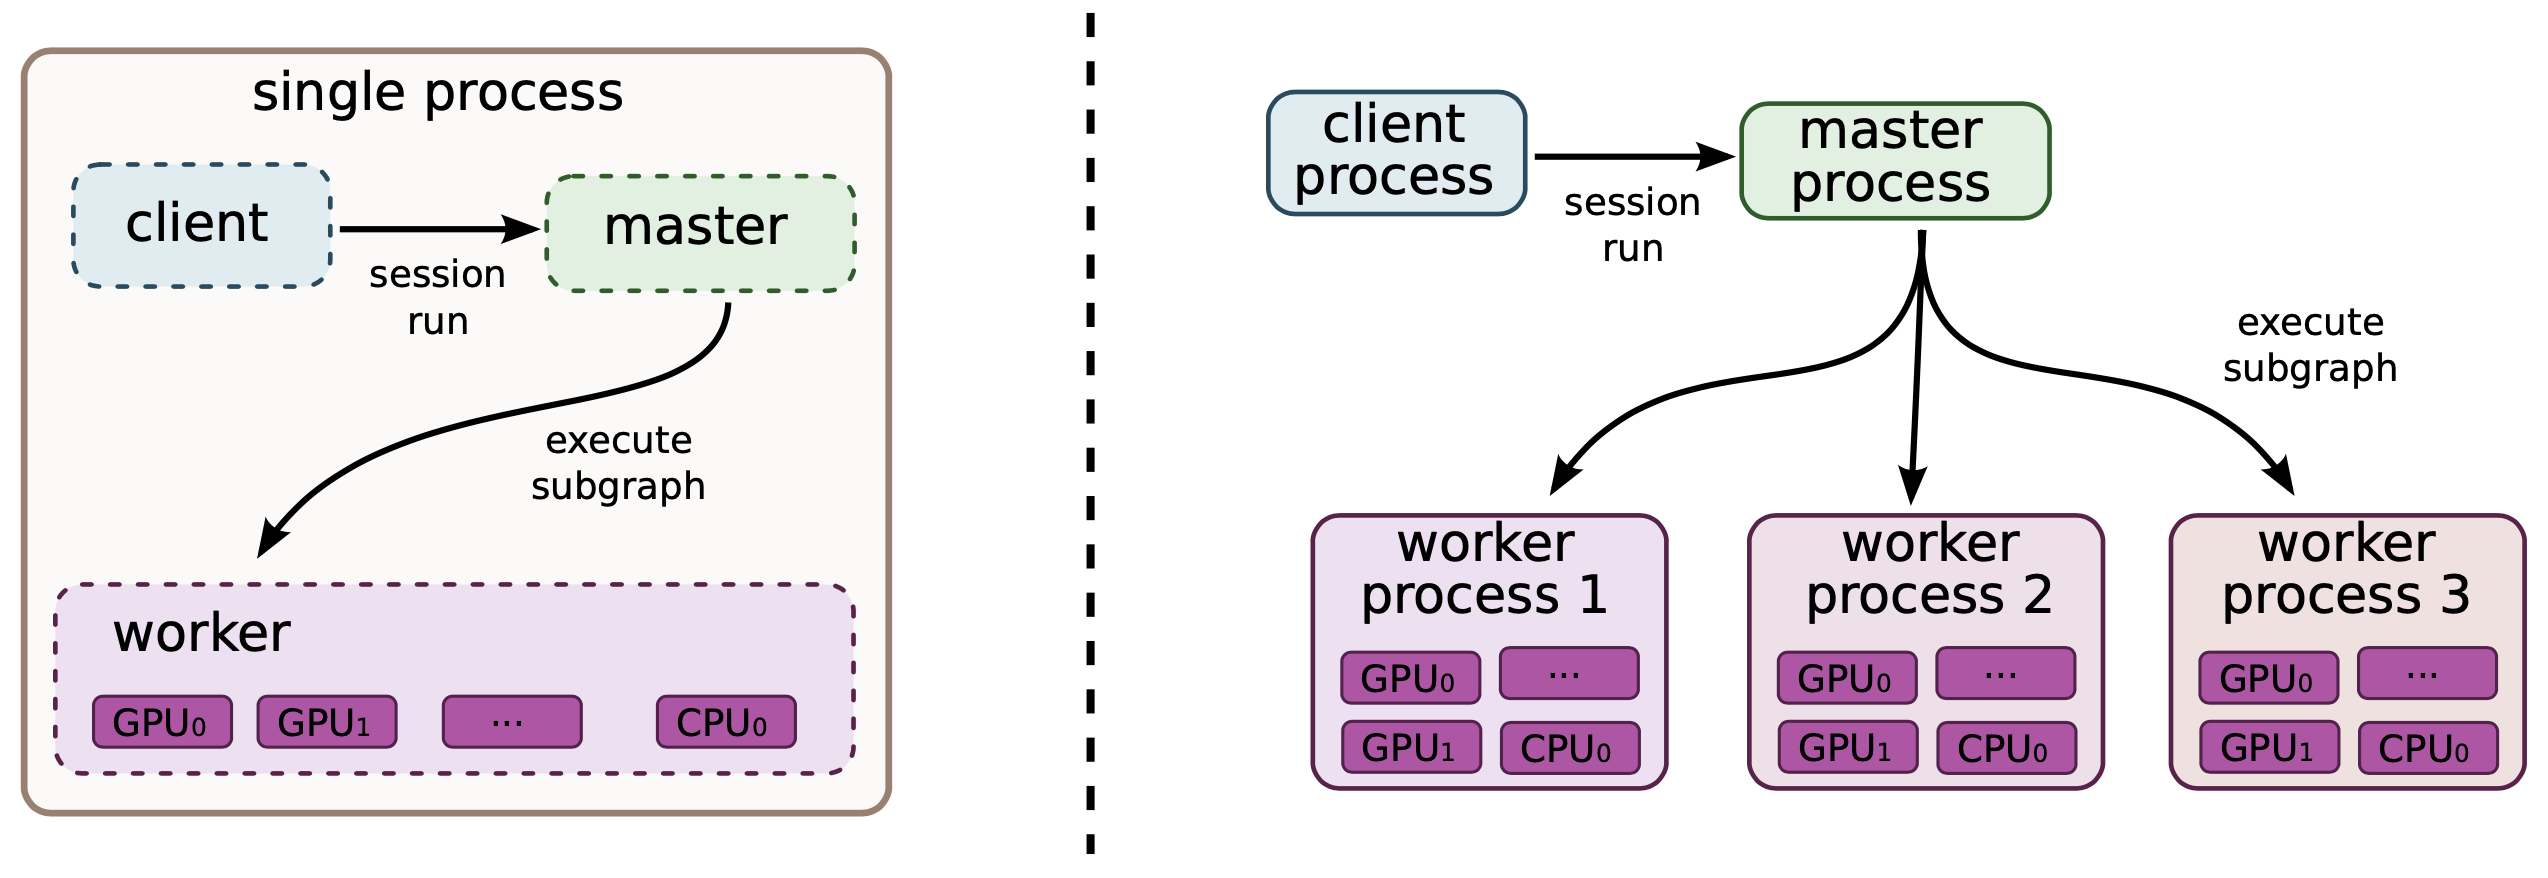
\includegraphics[width=\textwidth]{tf_dev.png}
    \caption{Схема работы TensorFlow с одной и несколькими машинами}
    \label{fig:tf_dev}
\end{figure}

При наличии нескольких вычислительных устройств появляется ряд проблем: принятие
решения о целевом устройстве для каждой вершины, коммуникация между устройствами.

Алгоритм, принимающий решение о размещении вершины на устройстве, учитывает
модель стоимости операций, которая оценивает время исполнения алгоритма и
объем требуемой памяти. Эта модель строится либо на основе эвристик, либо
по результатам предыдущих вычислений. Алгоритм размещения производит симуляцию
вычислений на графе, начиная во входных вершинах и продвигаясь вглубь. Для
каждой вершины, которая рассматривается алгоритмом, определяется список устройств,
на которых она может быть исполнена. В случае, если устройств больше 1,
используется жадный алгоритм, определяющий наиболее подходящее устройство.
Подробнее эти механизмы описаны в разделах 3.2.1 и 4.6 \cite{Abadi2016}.

По окончании размещения вершин происходит деление графа на подграфы. Каждый
подграф выполняется на 1 устройстве. Для обеспечения коммуникации между
устройствами, на границах подграфов вставляются служебные вершины передачи и
приема (англ. \textit{send and receive nodes}).

\begin{figure}[h]
    \centering
    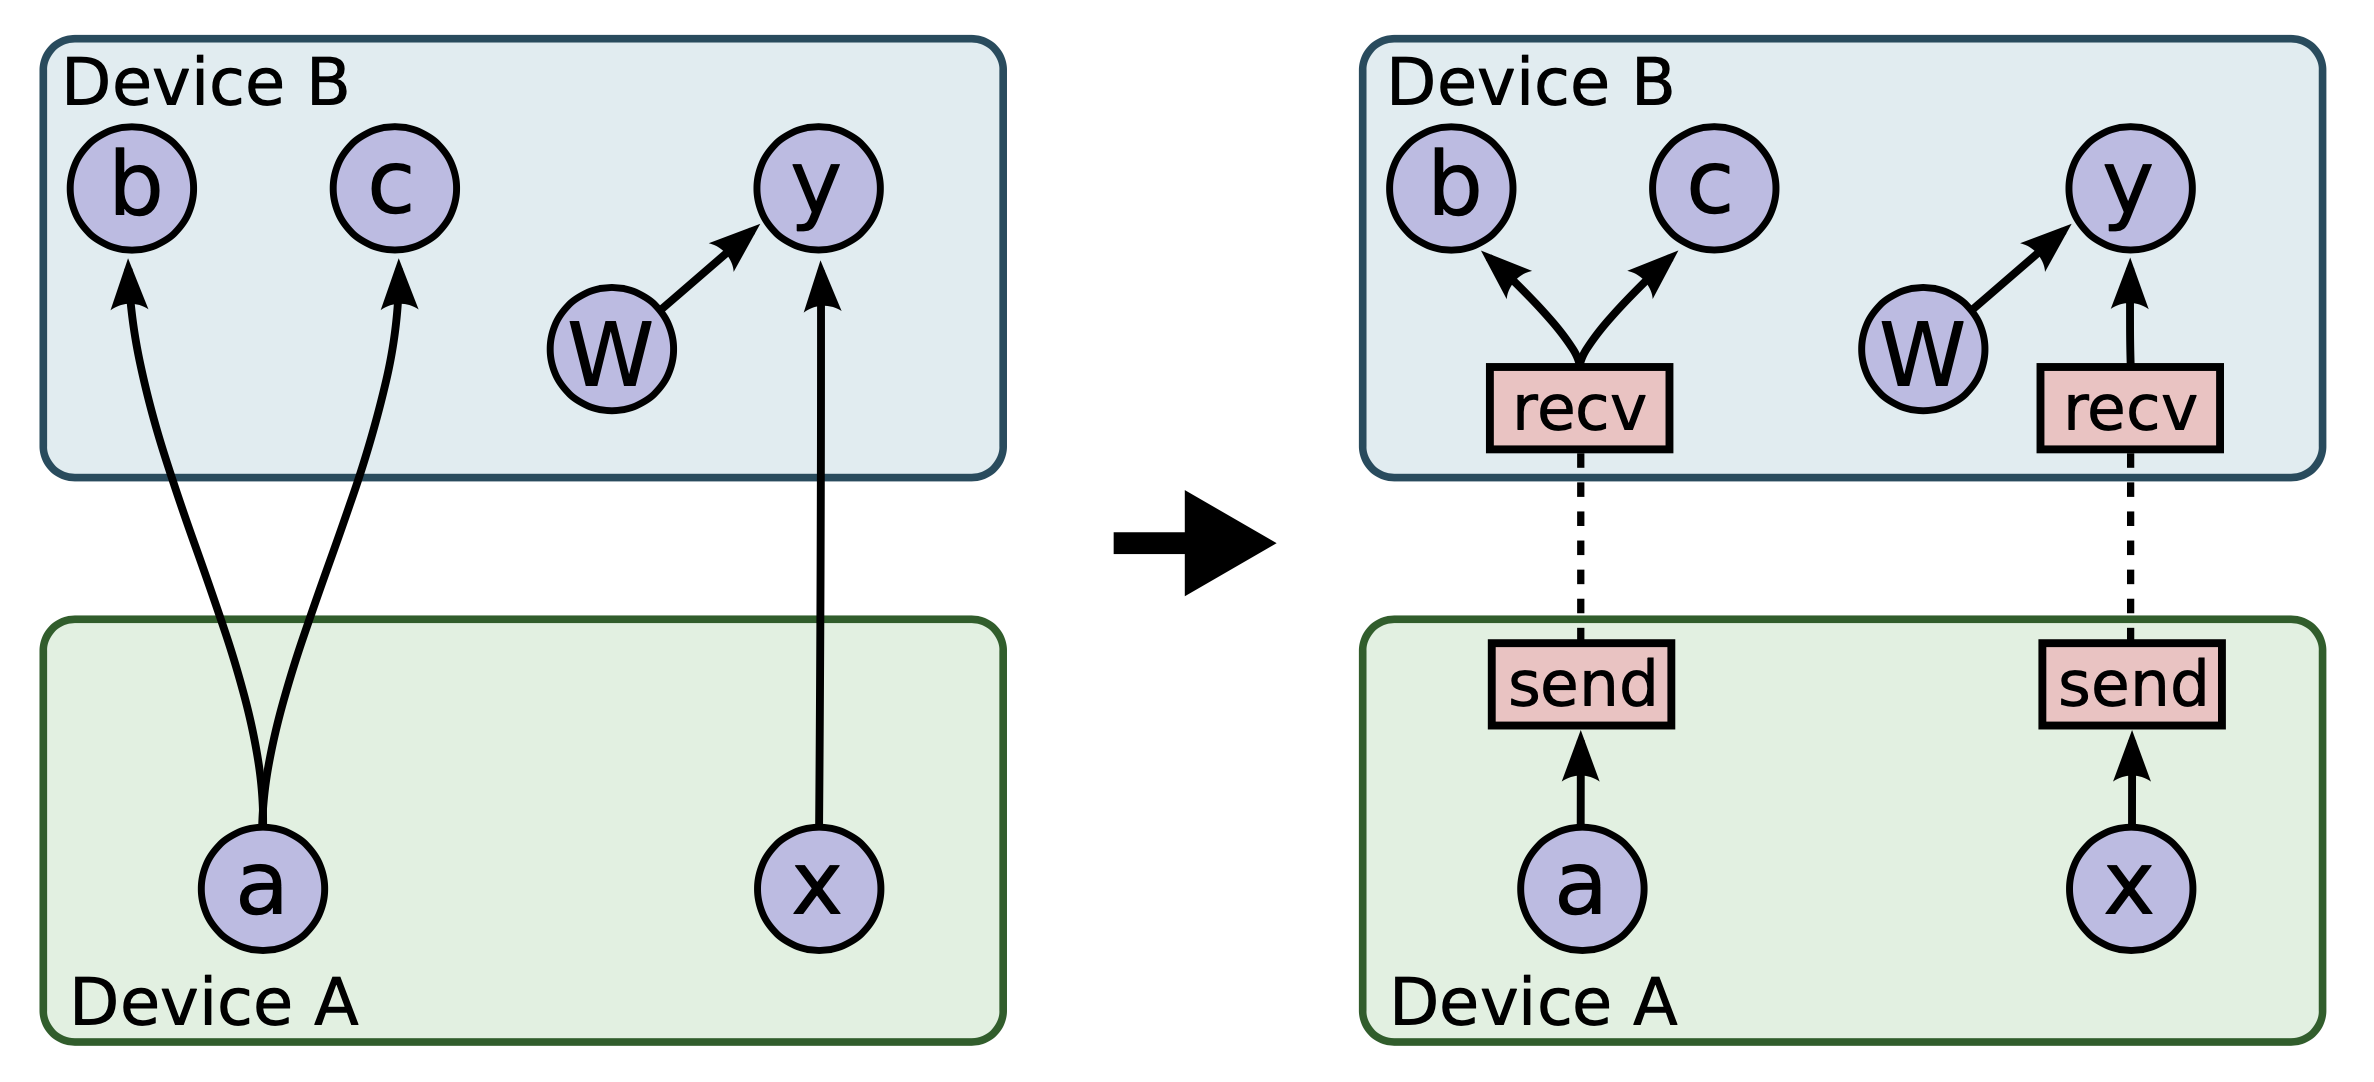
\includegraphics[width=\textwidth]{tf_graph_partition}
    \caption{Граф до и после деления на подграфы}
    \label{fig:tf_graph_partition}
\end{figure}

\subsubsection{Вычисление градиента на графе}

В TensorFlow реализована поддержка автоматического вычисления градиента функции.
Градиент вычисляется так же, как и любые другие функции, путем вычислений на
графе. Для построения необходимого графа используется следующая процедура.

Когда TensorFlow необходимо вычислить градиент тензора $C$ по некоторому
тензору $I$, от которого $C$ зависит, фреймворк сперва находит путь из
$I$ в $C$. Затем, начиная с конца этого пути (то есть из вершины, содержащей $C$),
библиотека добавляет в граф вершину, вычисляющую частную производную,
руководствуясь правилом дифференцирования сложной функции. Каждая операция сама
определяет правила собственного дифференцирования.

\begin{figure}[h]
    \centering
    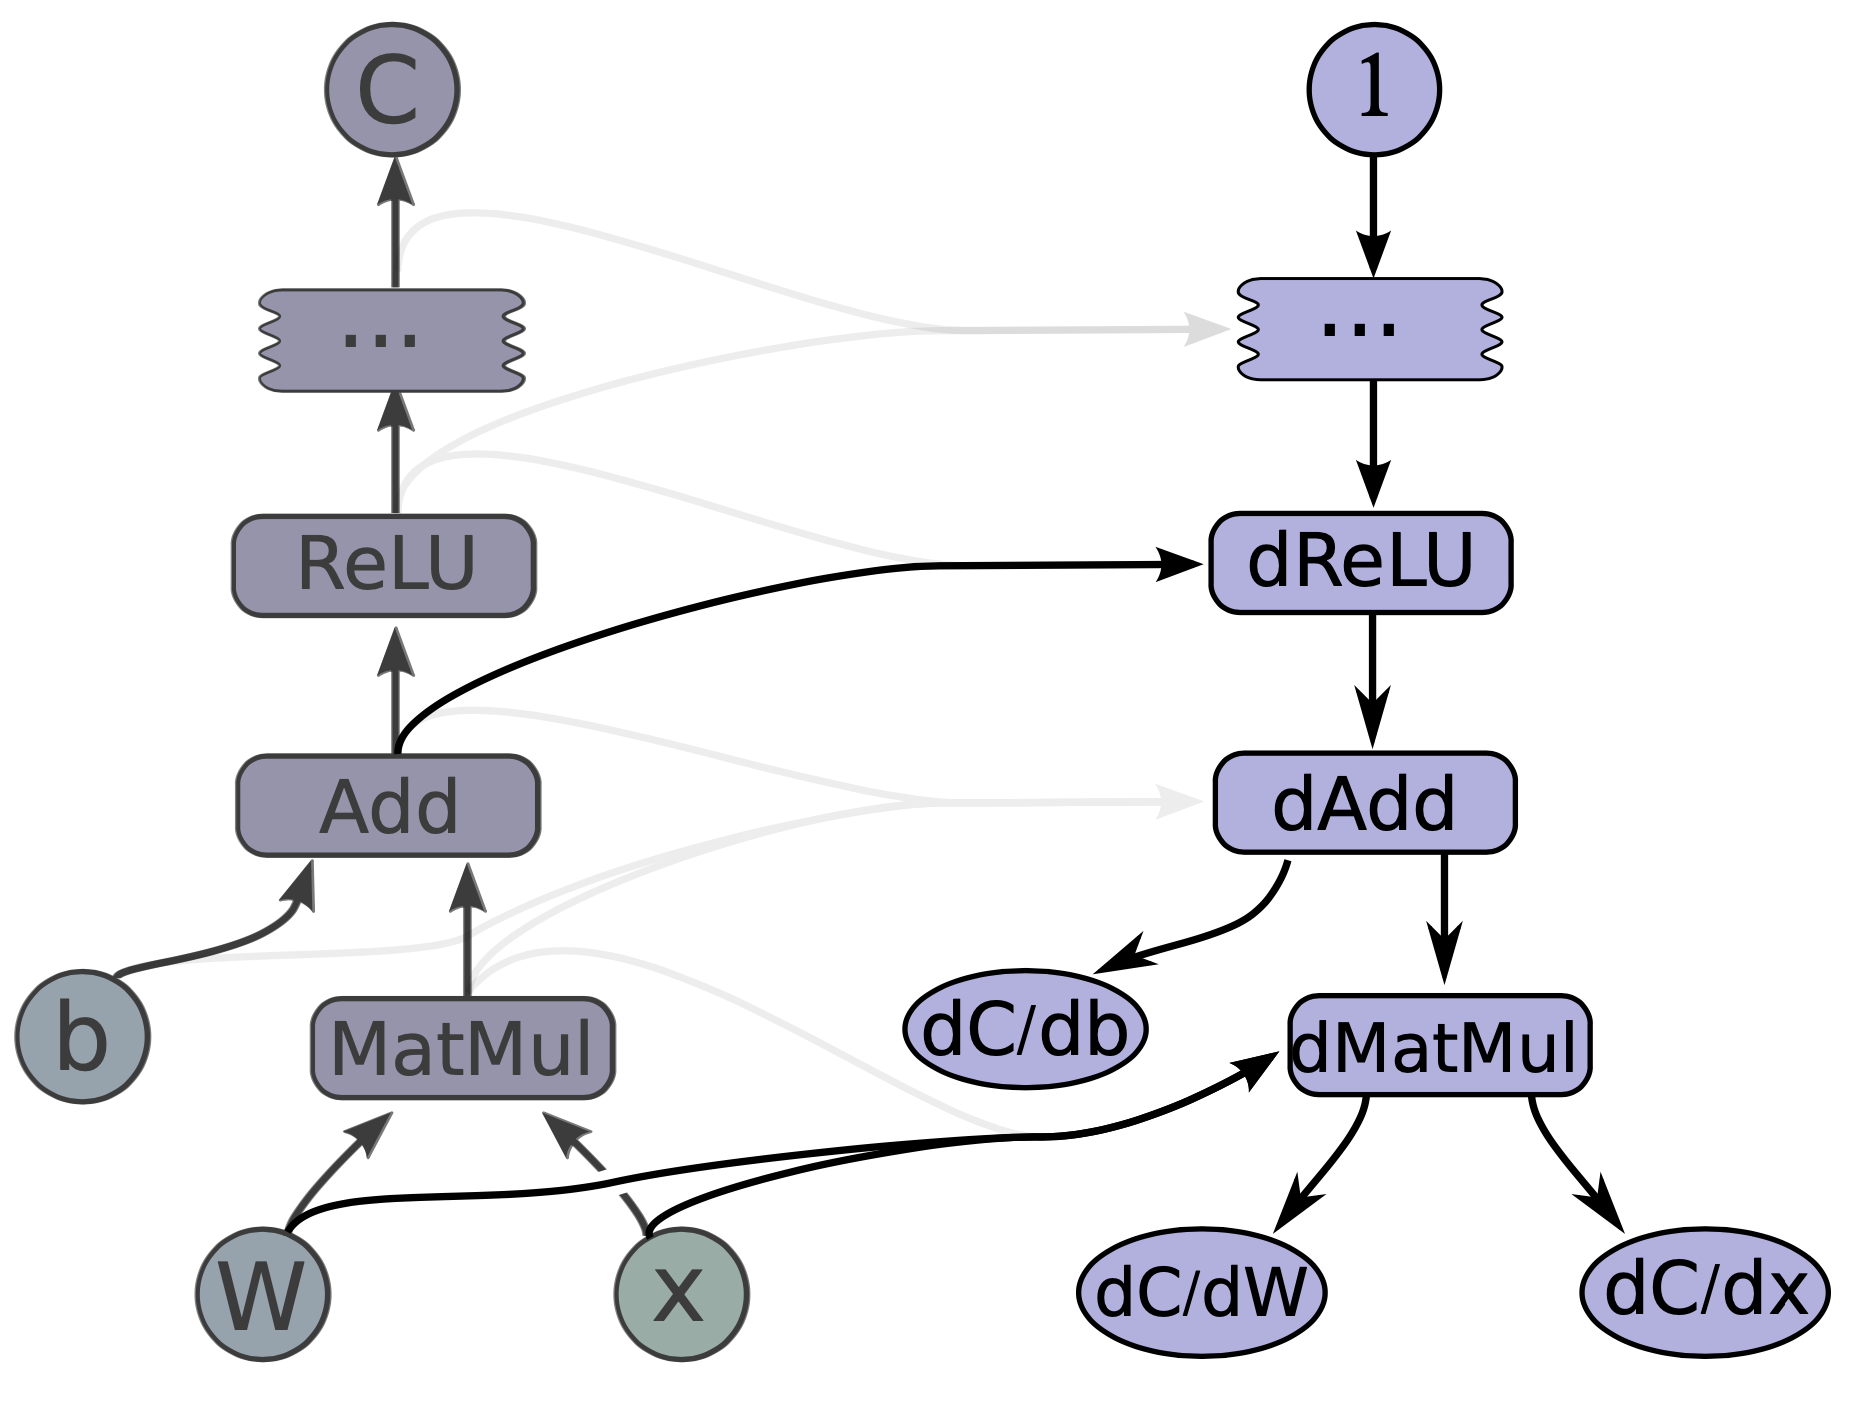
\includegraphics[width=0.5\textwidth]{tf_autograd}
    \caption{Работа алгоритма автоматического дифференцирования}
    \label{fig:tf_autograd}
\end{figure}

В общем случае, у операции может быть несколько выходов, а $C$ может зависеть
только от некоторых из них.

Автоматическое дифференцирование затрудняет работу оптимизационных процедур,
в частности анализ расхода памяти. У пользователя отсутствует возможность
управлять автоматически сгенерированной частью графа. Поскольку градиентные
вершины меняют направление вычислений, тензоры, которые использовались в начале,
зачастую требуются в конце. Это сильно ограничивает размер возможных вычислений,
в особенности на GPU.

\subsubsection{Частичное исполнение}

Часто необходимо вычислить только часть графа. Поэтому фреймворк предоставляет
возможность вычислять только отдельный подграф.

У каждой вершины в графе есть имя, а каждый выход вершины идентифицируется парой
<<имя:порт>>, где порт -- число от 0 до количества выходов. Граф преобразуется
таким образом, что каждая входная пара <<имя:порт>> дополняется вершиной
<<подачи>> (англ. \textit{feed node}), а выходящая -- вершиной <<получения>>
(англ. \textit{fetch node}). Затем используется описанный ранее алгоритм
определения вершин, которые необходимы для вычисления значения графа.

% \begin{figure}[h]
%     \centering
%     \includegraphics[width=0.4\textwidth]{tf_feed_fetch}
%     \caption{Граф до и после добавления специальных вершин}
%     \label{fig:tf_feed_fetch}
% \end{figure}

\subsubsection{Управление потоком выполнения}

Концепция управления потоком выполнения в TensorFlow похожа на ту, что
используется в машине потока данных с тегами-токенами MIT (англ.
\textit{MIT tagged-token dataflow machine})\cite{Arvind1987}.
Каждая итерация цикла однозначно идентифицируется меткой (тегом), а состояние
исполнения однозначно описывается фреймом.

В общем случае граф может содержать вершины, принадлежащие разным устройствам.
Таким образом, управление состоянием затрудняется проблемой определения момента
останова цикла. В качестве решения этой проблемы авторы предлагают дополнять
граф специальными управляющими вершинами.

\subsubsection{Операции входных вершин}

Хотя входные данные могут быть предоставлены графу посредством вершин <<подачи>>,
есть другой распространенный механизм, использующийся при обучении больших
распределенных моделей. Обычно таким вершинам предоставляется набор имен файлов.
Во время исполнения они производят один или более тензоров, содержащих образцы
для обучения. Это позволяет загружать данные напрямую с файловой системы. Если
клиент и рабочий процесс находятся на разных машинах, потребуется передача
данных по сети.

\subsection{Оптимизации}

\subsubsection{Выделение общей части выражения}
% todo translation?
Так как построение графа зачастую происходит путем комбинации нескольких слоев,
он может содержать лишние копирования результатов одних и тех же вычислений.
Для оптимизации ресурсов предусмотрен алгоритм выделения общей части выражений.
Этот алгоритм основан на результатах работы \cite{click}.

\subsubsection{Контроль обмена данными и расхода памяти}

Аккуратное размещение вершин на устройствах может привести к значительному
улучшению производительности. В частности, оптимальное планирование может
уменьшить промежуток времени, в течение которого необходимо хранить результаты
промежуточных вычислений.

Наиболее практичным авторы фреймворка видят оптимизацию планирования приемочных
вершин. Они могут начинать исполнение раньше, чем необходимо. Исследователи
анализируют критические пути в графе, чтобы оценить время выполнения вычислений.
Затем граф дополняется управляющими ребрами, откладывающими начало приема данных.

\subsubsection{Сжатие с потерями}

Некоторые алгоритмы машинного обучения, в частности те, что используются в
нейронных сетях, толерантны к шуму и снижению точности вычислений. Авторы
прибегают к сжатию данных с потерями при пересылке между устройствами. Например,
путем конвертации 32-битных чисел с плавающей точкой в 16-битные, а затем
выполняя обратные преобразования. Для этого граф дополняется специальными
вершинами.
